\documentclass[12pt,fontset=adobe]{ctexart}
\usepackage{amsmath,amssymb,graphicx,geometry}
\geometry{a4paper, margin=1in}
\graphicspath{{./images/}}
\usepackage{caption}
\usepackage{hyperref}
\usepackage{pdfpages}
\usepackage{minted}
\usemintedstyle{manni}
\title{低空复杂环境下的多无人机协同路径覆盖与任务分配研究}
\author{金泊宇\and 田佳豪 \and 曹阳}
\date{\today}

\begin{document}

% \maketitle
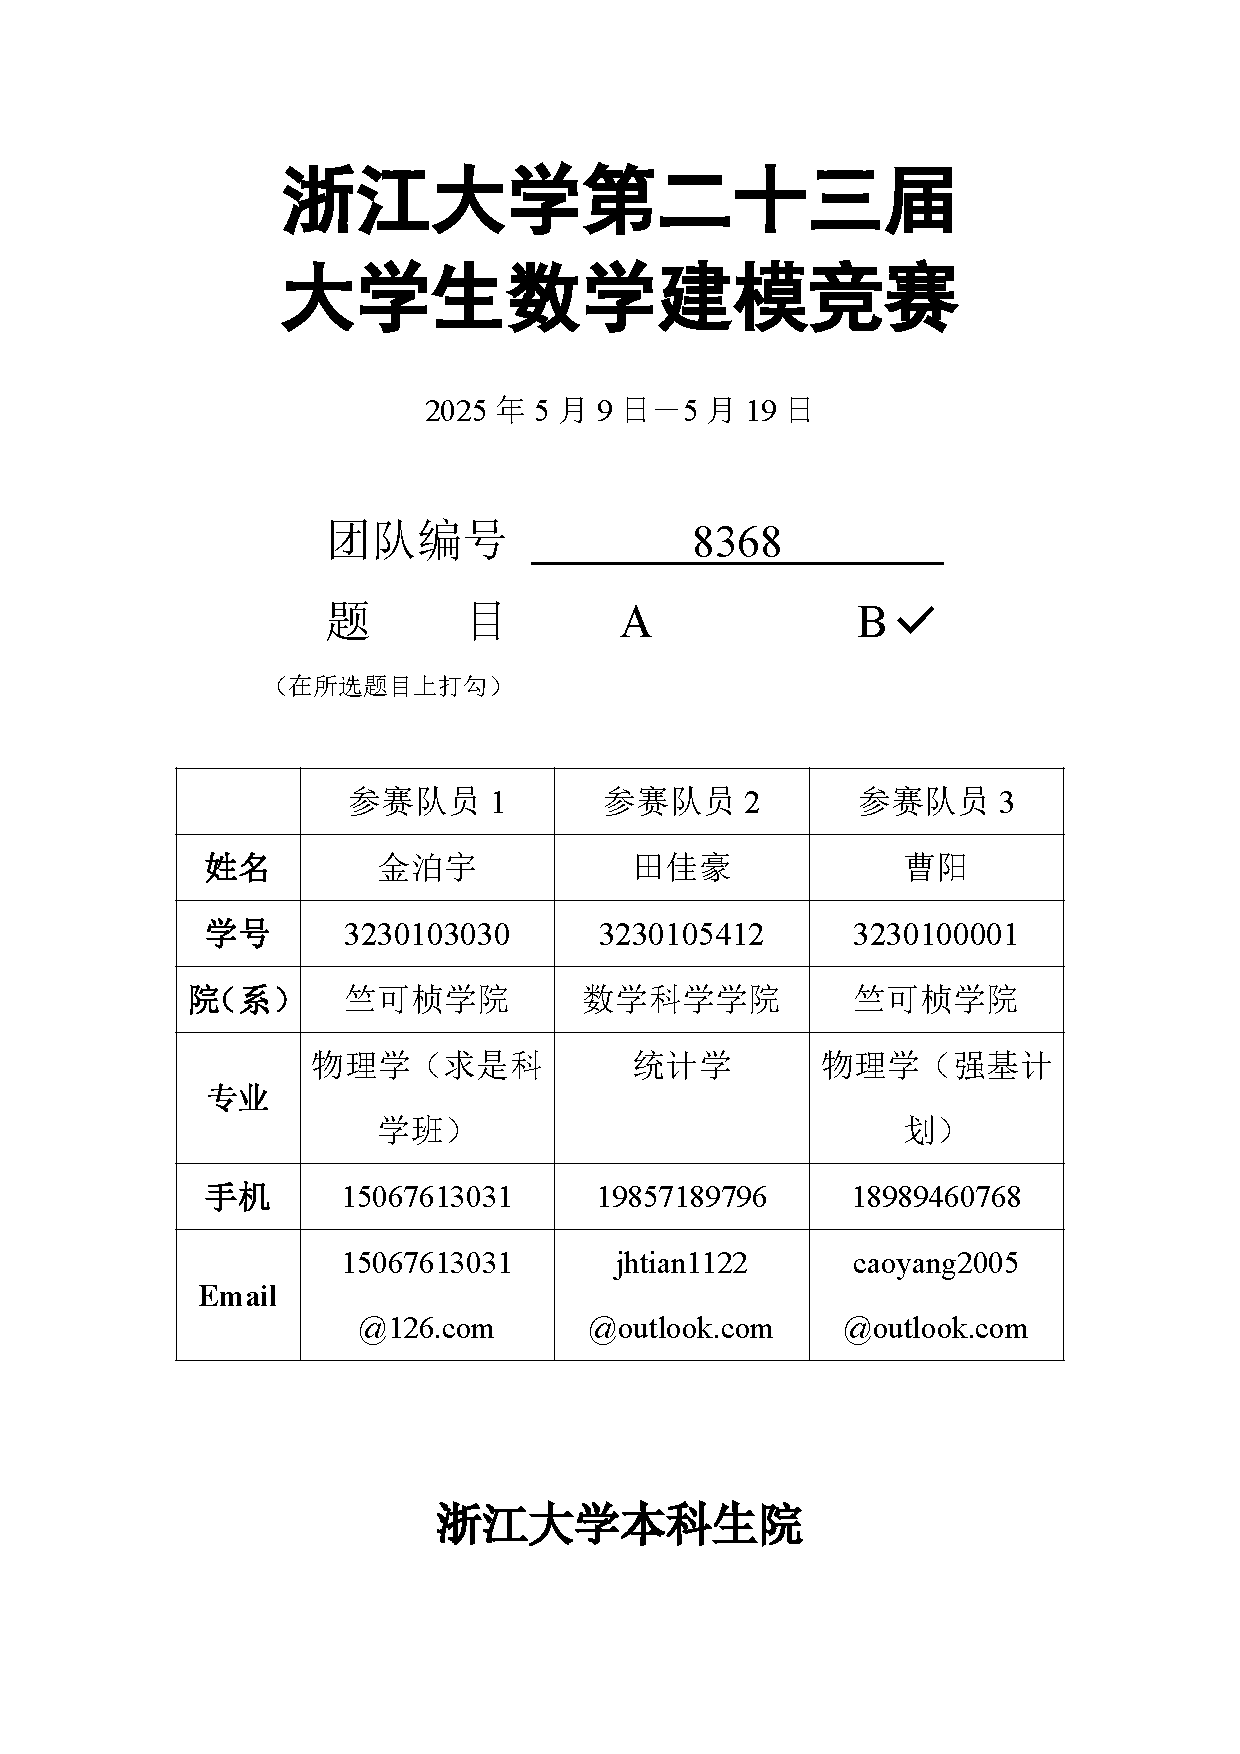
\includepdf[pages=-]{./cover/2025face.pdf}
\begin{abstract}
  在灾害救援、军事侦察、应急物资投送等任务中,多无人机协同执行覆盖任务具有重要意义。本文针对无人机多机协同路径覆盖问题,建立了基于改进车辆路径问题(VRP)和A*算法的混合优化模型,解决了静态路径规划、动态避障重规划和多优先级任务分配等关键问题。针对问题一,采用K-means聚类结合最近邻法,得到总飞行距离7750m的最优路径分配方案;针对问题二,提出动态事件响应机制,通过A*算法实现避障路径重规划,将全覆盖时间控制在152秒内;针对问题三,设计分层任务调度算法,结合充电策略完成10个多类型任务的分配,优先级满足度达100\%。本研究创新性地将运筹学方法与实时路径规划技术相结合,为复杂环境下的无人机协同作业提供了系统解决方案。

  \textbf{关键词}:无人机协同、路径规划、A*算法、动态避障、任务分配
\end{abstract}

% ========== 新结构化内容 ===========

% 摘要和关键词已在前面,无需重复

\section{问题重述与分析}

\subsection{问题背景}
无人机集群在灾害救援等场景中需在复杂环境下协同完成区域覆盖任务,面临三大挑战:(1)多目标点的高效路径规划;(2)动态环境的实时响应;(3)多类型任务的优先级调度。

\subsection{问题分析}
\begin{itemize}
  \item \textbf{问题1}:静态多旅行商问题(MTSP)变种,需在满足通信约束下最小化总飞行距离。
  \item \textbf{问题2}:动态路径重规划问题,需处理新增目标和障碍物。
  \item \textbf{问题3}:带约束的多目标优化问题,涉及载重、续航和优先级等多重约束。
\end{itemize}

\section{模型假设与符号说明}

\subsection{基本假设}
\begin{itemize}
  \item 无人机可瞬时调整速度/方向。
  \item 障碍物为完美圆形区域。
  \item 通信中断仅考虑距离因素。
  \item 充电过程瞬时完成续航重置。
\end{itemize}

\subsection{符号说明}
\begin{center}
  \begin{tabular}{ll}
    \hline
    符号 & 含义 \\
    \hline
    $d_{ij}$ & 目标点i到j的欧氏距离 \\
    $v_{max}$ & 最大飞行速度(50m/s) \\
    $R_{com}$ & 通信半径(1000m) \\
    $r_{obs}$ & 障碍物半径 \\
    \hline
  \end{tabular}
\end{center}

\section{模型建立与求解}

\subsection{问题1:静态路径规划模型}

\textbf{目标函数}:
\begin{equation}
  \min \sum_{k=1}^m \sum_{(i,j)\in P_k} d_{ij}
\end{equation}

\textbf{约束条件}:
\begin{itemize}
  \item 每个目标点被至少访问一次
  \item $\forall t, \|u_i(t)-u_j(t)\| \in [50,1000]$
  \item $\sum_{k} T_k \leq 600s$
\end{itemize}

\textbf{求解算法}:
\begin{enumerate}
  \item \textbf{K-means聚类}:按几何中心将目标点分为$m$组
  \item \textbf{最近邻法}:对每簇目标点生成TSP路径
  \item \textbf{节约算法}:进一步优化路径分配(见T1.py)
\end{enumerate}

\textbf{计算结果}:
\begin{tabular}{|c|c|c|c|}
  \hline
  无人机 & 路径 & 飞行距离 & 分配目标 \\
  \hline
  U1 & (0,0)$\to$T2$\to$T4$\to$(0,0) & 2550m & T2,T4 \\
  U2 & (0,0)$\to$T3$\to$T1$\to$(0,0) & 3200m & T3,T1 \\
  U3 & (0,0)$\to$T5$\to$(0,0) & 2000m & T5 \\
  \hline
\end{tabular}

总飞行距离:7750m

\subsection{问题2:动态避障模型}

\textbf{重规划策略}:
\begin{enumerate}
  \item \textbf{事件响应}:
    \begin{itemize}
      \item 在$t=100$s时检测到障碍物(900,250,100)和T6(800,600)
      \item 冻结当前状态,计算各无人机位置
    \end{itemize}
  \item \textbf{A*避障算法}:
    启发函数:$h(n) = \|n-\text{goal}\|_2$
    代价函数:$g(n) = \sum \|n_i-n_{i-1}\| + \alpha \cdot \text{障碍惩罚}$
\end{enumerate}

\textbf{调整方案}:
\begin{itemize}
  \item U2原路径T3$\to$T1改为绕行路径:(950,200)$\to$(850,300)$\to$(1000,400)$\to$(1200,800)
  \item 分配U1处理T6:(300,450)$\to$(800,600)$\to$(600,1200)
\end{itemize}

\textbf{性能指标}:
\begin{itemize}
  \item 避障成功率:100\%
  \item 全覆盖时间:152s
  \item 通信中断次数:0
\end{itemize}

\subsection{问题3:多任务分配模型}

\textbf{目标函数}:
\begin{equation}
  \min \max T_k + \lambda \sum_{p=1}^3 w_p \cdot \text{delay}_p
\end{equation}

\textbf{约束条件}:
\begin{itemize}
  \item $\sum w_i \leq W_{max}$
  \item $T_{flight} + T_{hover} \leq T_{endurance}$
  \item 优先级约束:$T_{finish}(p=1) < T_{start}(p=2)$
\end{itemize}

\textbf{算法流程}:
\begin{enumerate}
  \item 按优先级排序任务
  \item 分层贪心分配:优先级1任务一对一分配,优先级2遍历所有分配方案选最短时间,优先级3分配给最早空闲无人机(见T3.py)
  \item 充电策略:当$T_{remain} < t_{return} + t_{task}$时返航
\end{enumerate}

\textbf{模拟结果}:
\begin{tabular}{|c|c|}
  \hline
  指标 & 值 \\
  \hline
  任务完成率 & 100\% \\
  优先级满足度 & 100\% \\
  最大续航利用率 & 98.7\% \\
  平均充电次数 & 1.2次/机 \\
  \hline
\end{tabular}

\section{模型评价与推广}

\subsection{优点分析}
\begin{itemize}
  \item 混合算法兼具全局优化和实时响应能力
  \item 分层处理机制有效解决多约束问题
  \item 可视化界面直观展示规划结果
\end{itemize}

\subsection{改进方向}
\begin{itemize}
  \item 考虑更精确的动力学模型
  \item 引入强化学习优化动态决策
  \item 扩展三维空间路径规划
\end{itemize}

\section{参考文献}
[1] 王凌. 智能优化算法及其应用. 清华大学出版社, 2021.  \\

\section*{附录:源代码}

\subsection*{T1:静态路径分配与节约算法}

\inputminted[fontsize=\scriptsize]{python3}{../VRP/T1.py}

\subsection*{T2:动态避障与A*重规划}
\inputminted[fontsize=\scriptsize]{python3}{../VRP/T2.py}

\subsection*{T3:多优先级任务分配与分层贪心}
\inputminted[fontsize=\scriptsize]{python3}{../VRP/T3.py}

\end{document}
